% Created 2016-09-16 Fri 15:51
\documentclass[a4paper]{article}
\usepackage[utf8]{inputenc}
\usepackage[T1]{fontenc}
\usepackage{fixltx2e}
\usepackage{graphicx}
\usepackage{grffile}
\usepackage{longtable}
\usepackage{wrapfig}
\usepackage{rotating}
\usepackage[normalem]{ulem}
\usepackage{amsmath}
\usepackage{textcomp}
\usepackage{amssymb}
\usepackage{capt-of}
\usepackage{hyperref}
\usepackage[hyperref,x11names]{xcolor}
\usepackage[colorlinks=true,urlcolor=SteelBlue4,linkcolor=Firebrick4]{hyperref}
\author{Willian Ver Valen Paiva}
\date{\today}
\title{}
\hypersetup{
 pdfauthor={Willian Ver Valen Paiva},
 pdftitle={},
 pdfkeywords={},
 pdfsubject={},
 pdfcreator={Emacs 25.1.50.1 (Org mode 8.3.5)}, 
 pdflang={English}}
\begin{document}

\tableofcontents

\section{rapport TP2}
\label{sec:orgheadline13}
\subsection{the API}
\label{sec:orgheadline8}
\subsubsection{org.apache.hadoop.conf.Configuration}
\label{sec:orgheadline1}
class responssible to provide access to configuration parameters from the configuration directory
\subsubsection{org.apache.hadoop.conf.Configured}
\label{sec:orgheadline2}
Base class for things that may be configured with a Configuration.
\subsubsection{org.apache.hadoop.fs.FileSystem}
\label{sec:orgheadline3}
filesystem object to use the hadoop distributed file system
\subsubsection{org.apache.hadoop.fs.Path}
\label{sec:orgheadline4}
names a file or directoy in a FileSystem.
\subsubsection{org.apache.hadoop.io.IOUtils}
\label{sec:orgheadline5}
utility class responsible for the I/O related functionality
\subsubsection{org.apache.hadoop.util.Tool}
\label{sec:orgheadline6}
an interface to implement the handling of generic command-line options
\subsubsection{org.apache.hadoop.util.ToolRunner}
\label{sec:orgheadline7}
run classes that implement the tool interface

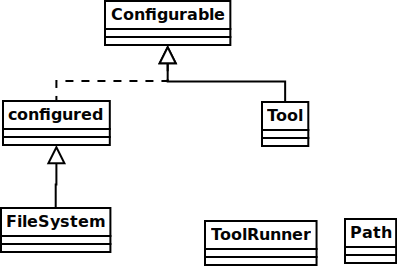
\includegraphics[width=.9\linewidth]{/home/willian/diagram.png}

\subsection{first and second program}
\label{sec:orgheadline11}
as the implementation of this program was given in class and the implementation is really similar
we take as best practice for the exercise explain the functionality of each step on the program
\subsubsection{the base}
\label{sec:orgheadline9}
the first step is to create a tool and implement the method run which will called on main in conjunction with ToolRunner
\subsubsection{the run method}
\label{sec:orgheadline10}
on the run method is where the program lives
the following is the steps followed to archive the functionality of the first program
\begin{enumerate}
\item create a URI object with the output path (file on the HDFS)
\item normalize the URI (means remove any "." ".." and etc)
\item create a Path object from the normalized URI
\item create a Configuration object and load the actual configuration on it via the command getConf
\item create a FileSystem object specifying the path, the configuration, and the user
\item create the outPutstream on the filesystem
\item create the inputstream usding the local file
\item copy the bytes from the inputstream to the outPutstream
\item close the streams
\end{enumerate}

for the second program the steps are really similar with the diference that on the step 7 and foward
has a litle change
\begin{enumerate}
\item create a loop for each local file
\item create the inputstream on the local file
\item copy the bytes from the inputstream to outPutstream
\item close the inputstream
\end{enumerate}
and after the loop close the outPutstream

\subsection{generation of words}
\label{sec:orgheadline12}
the implementation of this last exercise didn't differ much from the previous ones
to archive the goal 3 functions have being created :

\begin{verbatim}
public static char getRandom(char[] array) {
    int rnd = new Random().nextInt(array.length);
    return array[rnd];
}

public static String randomSyllable(){
    char[] alphabet = "abcdefghijklmnopqrstuvwxyz".toCharArray();
    return  new StringBuilder().append(getRandom(alphabet)).append(getRandom(alphabet)).toString();
}

public static String randomWord(int size){
    String exampleString = "";
    for(int i=0 ; i < size; i++){
        exampleString += randomSyllable();
    }
    return exampleString + " ";
 }
\end{verbatim}

them using the same code from the last exercise and changing the loop to iterate a number of times passed by argument
and changing how the inputstream is created :
\begin{verbatim}
InputStream is = new ByteArrayInputStream(randomWord(10).getBytes(StandardCharsets.UTF_8));
\end{verbatim}
that way reading the bytes direct from the string and not a file


\section{problems faced}
\label{sec:orgheadline14}
during the work no IDE was used and all the compilation and packaging was done using maven direct without a middle man
avoiding the problems of building 
\end{document}